\documentclass[11pt, a4paper]{article}

% --- Packages ---
\usepackage[utf8]{inputenc} % Encoding
\usepackage{amsmath, amssymb, amsthm} % Advanced math typesetting
\usepackage{physics} % Useful commands for physics (derivatives, vectors, braket)
\usepackage{graphicx} % For including diagrams and images
\usepackage{geometry} % Page margins
\usepackage{siunitx} % For proper formatting of SI units
\usepackage{fancyhdr} % Custom headers and footers
\usepackage{xcolor} % For blocks of color
\usepackage{enumitem} % For enumerated lists with letters
\usepackage{float} % For figure strict positioning
\usepackage{parskip} % Elimina la sangría y añade espacio entre párrafos
\usepackage{hyperref} % URL suppeort
\usepackage{tikz}
\usepackage{pgfplots}

% --- Page Setup ---
\geometry{top=2.5cm, bottom=2.5cm, left=2.5cm, right=2.5cm}
\pagestyle{fancy}
\fancyhf{} % Clear all default header and footer fields
\fancyhead[L]{\textbf{José Carlos López Henestrosa}}
\fancyhead[R]{Fundamentos físicos de la informática - Examen}
\fancyfoot[C]{\thepage} % Page number at the bottom center


% --- Custom Environments ---
% Creates a neat "Problem X" environment
% --- Custom Environments ---
\newenvironment{problem}[1][Cuestión]{
	\vspace{0.5cm}
	\noindent{\Large\bfseries #1} \par\vspace{0.5cm}
}{
	\vspace{0.5cm}
}

% --- Document Starts Here ---
\begin{document}
	% --- Title Block ---
	\begin{center}
		\Large{ \textbf{Examen} } \\
		\vspace{0.5cm}
		\normalsize{\textbf{Nombre:} José Carlos López Henestrosa} \\
	\end{center}

	\vspace{1cm}
	\hrule
	\vspace{1cm}

	% --- Exercise 1 ---
	\begin{problem}[Cuestión 1]
		Una onda electromagnética monocromática pasa de un gas a un cristal con un ángulo de incidencia de $45^{\circ}$ con la normal a la superficie que separa ambos medios. El índice de refracción del gas es $n_1 = 1,2$ y el del vidrio $n_2 = 1,8$. Responded a las siguientes preguntas:

		\begin{enumerate}[label=\alph*)] 
			\item ¿Cuál será el ángulo de refracción?

				{ \color{blue} 
					Para encontrar el ángulo de refracción, aplicamos la ley de Snell, que relaciona los índices de refracción de los dos medios con sus respectivos ángulos de incidencia y refracción:

					$$n_1 \text{ sen } \theta_1 = n_2 \text{ sen } \theta_2$$

					Sustituimos los datos que nos proporciona el enunciado ($n_1 = 1,2$; $\theta_1 = 45^{\circ}$; $n_2 = 1,8$):

					$$1,2 \cdot \text{sen}(45^{\circ}) = 1,8 \cdot \text{sen } \theta_2$$

					$$\text{sen } \theta_2 = \frac{1,2 \cdot \frac{\sqrt{2}}{2}}{1,8} = \frac{1,2 \cdot 0,7071}{1,8} = \frac{0,8485}{1,8} \approx 0,4714$$

					Despejamos el ángulo:
					$$\theta_2 = \text{arc sen}(0,4714) \approx 28,13^{\circ}$$

					El ángulo de refracción dentro del cristal será aproximadamente de \textbf{$28,13^{\circ}$}.
				}

			\item ¿Cómo varían la velocidad y la frecuencia de la onda al pasar de un medio a otro?

				{ \color{blue} 
					La \textbf{velocidad de propagación} de la onda luminosa es inversamente proporcional al índice de refracción del medio material ($v = \frac{c}{n}$). Puesto que la onda pasa de un gas con un índice menor ($n_1 = 1,2$) a un cristal con un índice mayor ($n_2 = 1,8$), el denominador en la expresión aumenta y, por lo tanto, la velocidad de propagación de la onda \textbf{disminuye}.

					La \textbf{frecuencia de la onda} electromagnética depende de la fuente emisora original y de los fotones que la componen ($E = hf$). Por lo tanto, la frecuencia se mantiene \textbf{constante} al atravesar la frontera entre los dos medios. No sufre ninguna variación.
				}
		\end{enumerate}
	\end{problem}

	% --- Exercise 2 ---
	\begin{problem}[Cuestión 2]
		En un experimento de doble rendija donde la pantalla se encuentra a una distancia $L = 1 \; \text{m}$, utilizamos luz verde ($\lambda_1 = 530 \; \text{nm}$) y se observa que la distancia entre los máximos de intensidad en el patrón de interferencia de la pantalla es 2,5 mm. Haciendo uso del mismo sistema, sustituimos la luz por luz violeta ($\lambda_2 = 410 \; \text{nm}$). Responded a las siguientes preguntas:

		\begin{enumerate}[label=\alph*)] 
			\item ¿Cuál será la nueva distancia entre franjas brillantes?

				{ \color{blue} 
					La distancia de separación entre los máximos consecutivos de interferencia ($\Delta y$) en la pantalla se define mediante la relación:
					$$\Delta y = \frac{\lambda L}{d}$$

					Dado que utilizamos exactamente el mismo sistema físico, la distancia a la pantalla ($L$) y la separación entre las dos rendijas ($d$) permanecen constantes. Esto nos permite establecer una relación de proporcionalidad directa matemática entre la separación de las franjas y la longitud de onda de la luz:
					$$\frac{\Delta y_1}{\lambda_1} = \frac{\Delta y_2}{\lambda_2}$$

					Despejamos la nueva separación $\Delta y_2$ y sustituimos los datos:

					$$\Delta y_2 = \Delta y_1 \frac{\lambda_2}{\lambda_1} = 2,5 \text{ mm} \cdot \frac{410 \text{ nm}}{530 \text{ nm}} = 2,5 \text{ mm} \cdot 0,7736 \approx 1,934 \text{ mm}$$

					Al cambiar a luz violeta, la cual tiene una longitud de onda menor, la nueva distancia entre las franjas brillantes se estrechará hasta ser de \textbf{$1,934 \text{ mm}$}.
				}

			\item Decid cuál es el fenómeno o los fenómenos que hacen aparecer las franjas y describidlos brevemente.

				{ \color{blue} 
					Cuando el frente de onda luminosa se encuentra con el obstáculo que suponen las dos rendijas, en lugar de seguir propagándose rectilíneamente, la onda se desvía y el frente se abre. De este modo, cada una de las dos rendijas actúa como una nueva fuente puntual de luz que emite ondas coherentes en varias direcciones. Este fenómeno se llama \textbf{difracción}.

					Por otro lado, las ondas difractadas provenientes de ambas rendijas viajan por el espacio y se superponen al llegar a la pantalla, cumpliendo así el principio de superposición. En aquellos puntos donde la diferencia de los caminos recorridos por las ondas es un múltiplo exacto de la longitud de onda ($\Delta r = m\lambda$), ambas llegan en fase y producen una \textbf{interferencia constructiva}, lo que forma los máximos de intensidad o franjas brillantes. Asimismo, donde llegan desfasadas, se anulan, lo cual genera zonas oscuras intermedias. Esto se trata de \textbf{interferencia destructiva}.
				}
		\end{enumerate}
	\end{problem}

	 % --- Exercise 3 ---
	\begin{problem}[Cuestión 3]
		Un circuito eléctrico está formado por una fuente de tensión constante V = 24 V, una resistencia R = 8 $\Omega$, una bobina de inductancia L = 2 H y un interruptor que se encuentra inicialmente abierto. Todos los elementos están en serie. En el instante t = 0, se cierra el interruptor para permitir el paso de la corriente.

		\begin{enumerate}[label=\alph*)] 
			\item Dibujad el circuito descrito en el enunciado.

				{ \color{blue} 
					\begin{center}
						\begin{circuitikz}[american, scale=1.2]
							\draw (0,0) to[battery, l=$V{=}24\text{ V}$] (0,3)
									to[switch, l=$t{=}0$] (2,3)
									to[R, l=$R{=}8\;\Omega$] (5,3)
									to[L, l=$L{=}2\text{ H}$] (5,0)
									-- (0,0);
						\end{circuitikz}
					\end{center}
				}

			\item ¿Cuál es la constante de tiempo del circuito?

				{ \color{blue}
					La constante de tiempo $\tau$ para un circuito inductivo-resistivo (RL) en serie se calcula dividiendo la inductancia entre la resistencia:

					$$\tau = \frac{L}{R} = \frac{2 \text{ H}}{8 \; \Omega} = 0,25 \text{ s}$$
				}

			\item Encontrad la expresión de la intensidad \textit{i(t)} para todo instante $t \ge 0$.

				{ \color{blue}
					Al cerrar el interruptor, el circuito comienza a cargarse y la corriente se incrementa según una curva exponencial. La expresión de la intensidad temporal para un circuito RL es:

					$$i(t) = \frac{V}{R} \left(1 - e^{-\frac{t}{\tau}}\right)$$

					Sustituimos los valores del circuito:

					$$i(t) = \frac{24}{8} \left(1 - e^{-\frac{t}{0,25}}\right) = 3 \left(1 - e^{-4t}\right) \text{ A}$$
				}

			\item Determinad el valor de la intensidad de corriente que circulará por el circuito cuando se haya alcanzado el régimen permanente.

				{ \color{blue}
					Al llegar al régimen permanente ($t \to \infty$), la bobina se carga magnéticamente por completo y pasa a comportarse como un cortocircuito ideal frente a la corriente continua. Por tanto, deja de oponerse al flujo de electrones y la intensidad máxima queda limitada por la resistencia:
					$$I = \frac{V}{R} = \frac{24 \text{ V}}{8 \; \Omega} = 3 \text{ A}$$
				}
		\end{enumerate}
	\end{problem}

	% --- Exercise 4 ---
	\begin{problem}[Cuestión 4]
		Tenemos el circuito de la siguiente figura:

		\begin{figure}[H]
			\centering
			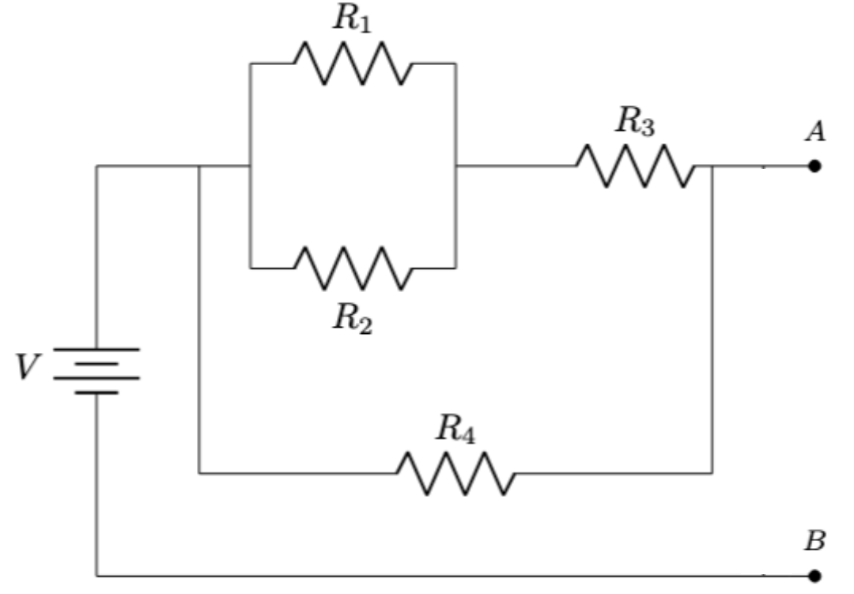
\includegraphics[width=14cm]{imagenes_entrega_latex/cuestion-4.png}
			\caption{Circuito de la Cuestión 4}
		\end{figure} 

		Con V = 30 V, $R_1 = 20 \; \Omega$, $R_2 = 30 \; \Omega$, $R_3 = 8 \; \Omega$ y $R_4 = 20 \; \Omega$.

		\begin{enumerate}[label=\alph*)] 
			\item Calculad la resistencia $R_{\text{Th}}$ y la tensión $V_{\text{Th}}$ del equivalente de Thevenin del circuito.

				{ \color{blue}                 
					Para hallar la resistencia de Thévenin ($R_{\text{Th}}$), sustituimos la fuente de tensión por un cortocircuito y calculamos la resistencia equivalente vista desde los terminales A y B:

					Las resistencias $R_1$ y $R_2$ se encuentran en paralelo:
					$$R_{12} = \frac{R_1 \cdot R_2}{R_1 + R_2} = \frac{20 \cdot 30}{20 + 30} = \frac{600}{50} = 12 \; \Omega$$

					Esta combinación se sitúa en serie con $R_3$:
					$$R_{123} = R_{12} + R_3 = 12 + 8 = 20 \; \Omega$$

					Finalmente, toda la rama superior queda en paralelo con $R_4$:
					$$\boxed{R_{\text{Th}} = \frac{R_{123} \cdot R_4}{R_{123} + R_4} = \frac{20 \cdot 20}{20 + 20} = \frac{400}{40} = 10 \; \Omega}$$

					Para calcular la tensión de Thévenin ($V_{\text{Th}}$), al estar los terminales A y B completamente en abierto, no existe un camino cerrado y, por tanto, no circula corriente a través de la red de resistencias. Al no haber intensidad, la caída de tensión en el conjunto de resistencias es nula. En consecuencia, la tensión medida entre A y B será exactamente la que proporciona la fuente:
					$$\boxed{V_{\text{Th}} = V = 30 \text{ V}}$$
				}

			\item Dibujad el circuito equivalente de Thevenin.

				{ \color{blue} 
					\begin{center}
						\begin{circuitikz}[american, scale=1.2]
							\draw (0,0) to[battery, l=$V_{\text{Th}}{=}30\text{ V}$] (0,2)
									to[R, l=$R_{\text{Th}}{=}10\;\Omega$] (4,2)
									node[ocirc, label=above:$A$] {};
							\draw (0,0) -- (4,0) node[ocirc, label=above:$B$] {};
						\end{circuitikz}
					\end{center}
				}

			\item Si se cortocircuitara la resistencia $R_4$, ¿cómo cambiaría la resistencia total del circuito? ¿Y la intensidad total? Razonad la respuesta.

				{ \color{blue} 
					Si se cortocircuita $R_4$, se está introduciendo una vía de resistencia nula en paralelo con el resto de la rama superior resistiva ($R_{123}$).

					Por las propiedades de los circuitos en paralelo, la corriente escoge siempre el trayecto de menor oposición. Por ello, la \textbf{resistencia total equivalente del circuito} ($R_{\text{Th}}$) caería a \textbf{$0 \; \Omega$}, ya que el paralelo entre $20 \; \Omega$ y $0 \; \Omega$ es $0 \; \Omega$.

					Respecto a la \textbf{intensidad total}, al desaparecer por completo la resistencia que limitaba el paso de los electrones, la intensidad pasaría de su valor calculado en condiciones normales ($3 \text{ A}$) a aumentar exponencialmente hasta \textbf{tender a infinito}, lo que en la práctica originaría un cortocircuito directo sobre la fuente de alimentación de 30 V.
				}
		\end{enumerate}
	\end{problem}

	% -- Exercise 5 ---
	\begin{problem}[Cuestión 5]
		Indicad si las siguientes afirmaciones son \textit{ciertas} o \textit{falsas} y justificad la respuesta.

		\begin{enumerate}[label=\alph*)] 
			\item En una esfera conductora vacía y cargada en equilibrio electroestático, el campo eléctrico en el interior (zona vacía) es directamente proporcional a la carga total $Q$ depositada en la esfera.

				{ \color{blue}
					\textbf{Falsa.} Al tratarse de un material conductor en equilibrio electrostático, la carga neta se redistribuye y se acumula en las superficies externas. Por consiguiente, el campo eléctrico total en el interior del material conductor es \textbf{siempre nulo} ($\vec{E} = 0 \text{ N/C}$), con independencia del valor absoluto de la carga total $Q$ que se haya depositado en la esfera.
				}

			\item Cuando un material conductor se somete a un campo eléctrico externo, la polarización de sus átomos o moléculas genera un campo eléctrico interno proporcional al campo externo, reforzando así la intensidad del campo eléctrico total en el interior del material.

				{ \color{blue}
					\textbf{Falsa.} El enunciado mezcla erróneamente los conceptos de conductor y dieléctrico. La polarización de átomos o moléculas para formar pequeños dipolos eléctricos ocurre en los materiales dieléctricos o aislantes y el campo interno que generan se opone al campo externo aplicado, lo cual lo reduce en vez de reforzarlo. De forma contraria, en un material conductor sometido a un campo externo, los electrones libres se desplazan produciendo una reconfiguración de cargas. Esto genera un campo interno que compensa exactamente al campo exterior, lo que provoca que el campo eléctrico total en el interior se anule por completo.
				}
		\end{enumerate}
	\end{problem}

	% -- Exercise 6 ---
	\begin{problem}[Cuestión 6]
		Dos cargas puntuales están ubicadas en el vacío en las siguientes coordenadas cartesianas.

		\begin{itemize}
			\item $Q_1 = +3 \; \text{nC}$ en el origen de coordenadas $\vec{r_1} = 0 \vec{i} + 0 \vec{j} \; \text{m}$.
			\item $Q_2 = -1 \; \text{nC}$ en el punto $\vec{r_2} = 4 \vec{i} \; \text{m}$.
		\end{itemize}

		\begin{enumerate}[label=\alph*)]
			\item Determinad el vector campo eléctrico total $\vec{E}$ en el punto $P$ situado en $\vec{r}_P = \vec{i} + 2 \vec{j} \; \text{m}$.

				{ \color{blue}
					Para determinar el campo eléctrico total, aplicaremos el principio de superposición calculando el campo creado por cada carga de forma individual y sumando posteriormente de forma vectorial: $\vec{E}_T = \vec{E}_1 + \vec{E}_2$.

					Calculamos primero los vectores distancia entre las cargas y el punto $P$ junto con sus respectivos módulos:
					\begin{itemize}
						\item Para $Q_1$: $\mathbf{\vec{d}_1} = \vec{r}_P - \vec{r}_1 = (1\vec{i} + 2\vec{j}) - (0\vec{i} + 0\vec{j}) = \mathbf{\vec{i} + 2\vec{j} \textbf{ m}}$. 

						Su módulo es $\mathbf{d_1} = \sqrt{1^2 + 2^2} = \sqrt{5} \approx \mathbf{2,236 \textbf{ m}}$.

						\item Para $Q_2$: $\mathbf{\vec{d}_2} = \vec{r}_P - \vec{r}_2 = (1\vec{i} + 2\vec{j}) - (4\vec{i} + 0\vec{j}) = \mathbf{-3\vec{i} + 2\vec{j} \textbf{ m}}$. 

						Su módulo es $\mathbf{d_2} = \sqrt{(-3)^2 + 2^2} = \sqrt{9 + 4} = \sqrt{13} \approx \mathbf{3,606 \textbf{ m}}$.
					\end{itemize}

					Ahora calculamos el campo eléctrico generado por cada carga utilizando la constante eléctrica $\frac{1}{4\pi\varepsilon_0} \approx 8,99 \times 10^9 \text{ N}\cdot\text{m}^2/\text{C}^2$:

					\textbf{Campo creado por $Q_1 = 3 \text{ nC}$:}
					$\vec{E}_1 = (8,99 \times 10^9) \frac{3 \times 10^{-9}}{(\sqrt{5})^2} \left( \frac{1}{\sqrt{5}}\vec{i} + \frac{2}{\sqrt{5}}\vec{j} \right) \approx \mathbf{2,41 \vec{i} + 4,83 \vec{j} \textbf{ N/C}}$.

					\textbf{Campo creado por $Q_2 = -1 \text{ nC}$:}
					$\vec{E}_2 = (8,99 \times 10^9) \frac{-1 \times 10^{-9}}{(\sqrt{13})^2} \left( \frac{-3}{\sqrt{13}}\vec{i} + \frac{2}{\sqrt{13}}\vec{j} \right) \approx \mathbf{0,58 \vec{i} - 0,38 \vec{j} \textbf{ N/C}}$.

					\textbf{Campo total en $P$:}
					Sumamos ambas componentes vectoriales para obtener el campo eléctrico resultante:

					$$\vec{E}_T = (2,41 + 0,58)\vec{i} + (4,83 - 0,38)\vec{j} = \mathbf{2,99 \vec{i} + 4,45 \vec{j} \textbf{ N/C}}$$
				}

			\item El potencial eléctrico en el punto $P$.

				{ \color{blue}
					El potencial eléctrico total en $P$ es una magnitud escalar que se halla sumando los potenciales individuales generados por cada carga en dicho punto. Consideramos el infinito como el origen de los potenciales. 

					$V_P = V_1 + V_2 = \frac{1}{4\pi\varepsilon_0} \left( \frac{Q_1}{d_1} + \frac{Q_2}{d_2} \right)$

					Evaluamos cada potencial utilizando las distancias obtenidas en el apartado anterior:

					\textbf{Potencial creado por $Q_1$:}
					$V_1 = (8,99 \times 10^9) \frac{3 \times 10^{-9}}{\sqrt{5}} \approx \mathbf{12,06 \text{ V}}$.

					\textbf{Potencial creado por $Q_2$:}
					$V_2 = (8,99 \times 10^9) \frac{-1 \times 10^{-9}}{\sqrt{13}} \approx \mathbf{-2,49 \text{ V}}$.

					\textbf{Potencial total en $P$:}
					$V_P = 12,06 \text{ V} - 2,49 \text{ V} = \mathbf{9,57 \text{ V}}$.
				}
		\end{enumerate}
	\end{problem}


	% --- Cuestión 7 ---
	\begin{problem}[Cuestión 7]
		Un conductor cilíndrico muy largo (que puede considerarse infinito) tiene un radio R = 2 cm. Por este conductor circula una intensidad de corriente total $I = 10 \; \text{A}$, distribuida de forma uniforme por toda su sección transversal.

		\begin{enumerate}[label=\alph*)] 
			\item Encontrad la expresión para el campo de inducción magnética $B$ exterior al conductor cilíndrico, en función de la distancia $r$ respecto al eje central del cilindro.

				{ \color{blue} 
					Para calcular el campo magnético en el exterior del cilindro, dado que existe una simetría cilíndrica, podemos aplicar el teorema de Ampère considerando una curva cerrada circular de radio $r > R$ concéntrica al cilindro. El comportamiento del campo exterior es idéntico al de un hilo infinito por el que circula la misma intensidad total $I$. La expresión para el módulo del campo de inducción magnética exterior es:
					\begin{equation*}
						B(r) = \frac{\mu_0 I}{2\pi r}
					\end{equation*}
					donde $\mu_0$ es la permeabilidad magnética del vacío. Vectorialmente, la dirección del campo da vueltas alrededor del cilindro.
				}

			\item Determinad el valor del campo de inducción magnética en un punto situado a $r = 3 \; \text{cm}$ del eje del conductor.

				{ \color{blue} 
					Dado que el punto se encuentra a $r = 3 \text{ cm}$ y el radio del cilindro es $R = 2 \text{ cm}$, estamos analizando un punto en la región exterior al conductor, ya que $r > R$. Podemos aplicar directamente la expresión hallada en el apartado anterior. 

					Sustituyendo el valor de la distancia $r = 0,03 \text{ m}$, la corriente $I = 10 \text{ A}$ y la permeabilidad $\mu_0 = 4\pi \times 10^{-7} \text{ T}\cdot\text{m/A}$:
					\begin{align*}
						B(0,03) &= \frac{4\pi \times 10^{-7} \cdot 10}{2\pi \cdot 0,03} \\
						&= \frac{2 \times 10^{-6}}{0,03} \\
						&= \frac{2}{3} \times 10^{-4} \approx \mathbf{6,67 \times 10^{-5} \text{ T}}
					\end{align*}
				}

			\item Ahora tenemos un hilo paralelo al conductor cilíndrico y a una distancia de 3 cm, por el que pasa una corriente $I_1 = 2 \; \text{A}$. Dibujad de forma esquemática la fuerza magnética entre el hilo y el conductor cilíndrico. ¿En qué caso sentirán una fuerza de atracción entre ellos? Justificad la respuesta.

				{ \color{blue} 
					Esquema de la fuerza magnética suponiendo el caso de atracción:

					\begin{center}
						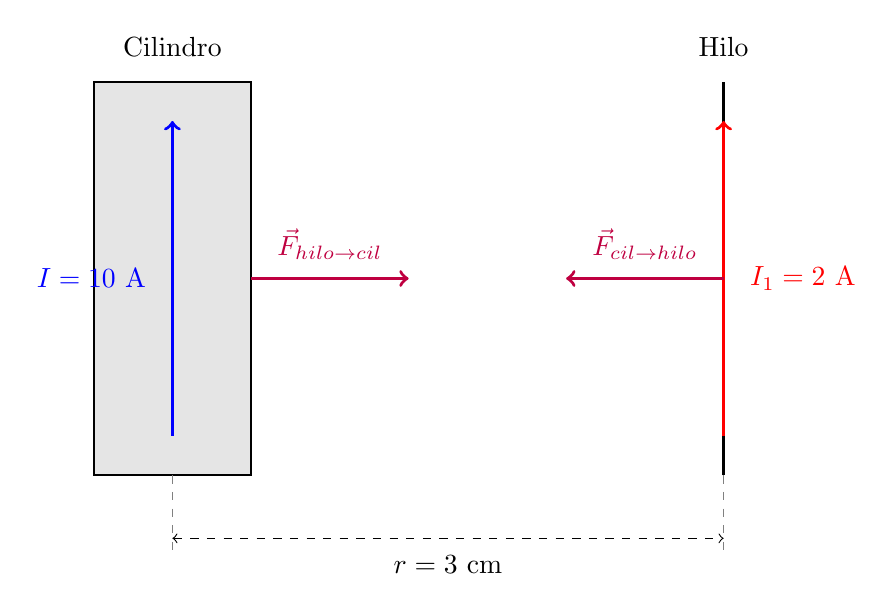
\begin{tikzpicture}
							% Cilindro conductor
							\draw[thick, fill=gray!20] (0,0) rectangle (2,5);
							\node[above] at (1, 5.2) {Cilindro};
							\draw[->, very thick, blue] (1, 0.5) -- (1, 4.5) node[midway, left=0.2cm] {$I = 10 \text{ A}$};

							% Hilo paralelo (separado para evitar superposición)
							\draw[very thick, black] (8,0) -- (8,5);
							\node[above] at (8, 5.2) {Hilo};
							\draw[->, very thick, red] (8, 0.5) -- (8, 4.5) node[midway, right=0.2cm] {$I_1 = 2 \text{ A}$};

							% Distancia (con líneas de referencia)
							\draw[dashed, gray] (1,0) -- (1,-1);
							\draw[dashed, gray] (8,0) -- (8,-1);
							\draw[<->, dashed] (1, -0.8) -- (8, -0.8) node[midway, below=0.1cm] {$r = 3 \text{ cm}$};

							% Fuerzas magnéticas (atracción) centradas en el espacio libre
							\draw[->, very thick, purple] (2, 2.5) -- (4, 2.5) node[midway, above=0.1cm] {$\vec{F}_{hilo \to cil}$};
							\draw[->, very thick, purple] (8, 2.5) -- (6, 2.5) node[midway, above=0.1cm] {$\vec{F}_{cil \to hilo}$};
						\end{tikzpicture}
					\end{center}

					El conductor cilíndrico y el hilo paralelo sentirán una \textbf{fuerza de atracción solo en el caso de que ambas intensidades circulen en el mismo sentido}.

					Según la regla de la mano derecha, la corriente del cilindro genera a su alrededor un campo de inducción magnética. En la posición del hilo, este campo perpendicular ejerce una fuerza de Lorentz sobre las cargas en movimiento del hilo. Si ambas corrientes fluyen en la misma dirección, el producto vectorial resultante de la velocidad de las cargas en el hilo y el campo magnético externo apuntará directamente hacia el cilindro, generando así una atracción mutua. No obstante, si circulasen en sentidos opuestos, la fuerza experimentada sería de repulsión.
				}
		\end{enumerate}
	\end{problem}


	% --- Cuestión 8 ---
	\begin{problem}[Cuestión 8]
		Un diodo a una temperatura T = 300 K tiene una corriente de saturación en inversa de $I_S = 2 \; \text{pA}$.

		\begin{enumerate}[label=\alph*)] 
			\item Encontrad la intensidad que pasa por $V = 0,5 \; \text{V}$.

				{ \color{blue} 
					La intensidad que atraviesa un diodo en función del voltaje de polarización $V$ viene dada por la expresión característica del diodo:

					\begin{equation*}
						I(V) = I_S \left( e^{\frac{qV}{k_B T}} - 1 \right)
					\end{equation*}

					Sabiendo que la magnitud inversa de la fracción es el potencial térmico, el cual se nos indica que a $T = 300 \text{ K}$ tiene un valor de $\frac{k_B T}{q} = 0,026 \text{ V}$, podemos reescribir la fórmula y sustituir los datos proporcionados: el voltaje $V = 0,5 \text{ V}$ y la corriente de saturación $I_S = 2 \text{ pA} = 2 \times 10^{-12} \text{ A}$.

					\begin{align*}
						I(0,5) &= 2 \times 10^{-12} \left( e^{\frac{0,5}{0,026}} - 1 \right) \\
						&= 2 \times 10^{-12} \left( e^{19,23} - 1 \right) \\
						&\approx 2 \times 10^{-12} \left( 2,248 \times 10^8 - 1 \right) \\
						&\approx \mathbf{4,50 \times 10^{-4} \text{ A}} = \mathbf{0,45 \text{ mA}}
					\end{align*}
				}

			\item Encontrad ahora la intensidad que pasa por el diodo para $V = -0,5 \; \text{V}$. Razonad el resultado.

				{ \color{blue} 
					Aplicamos de nuevo la fórmula característica del diodo pero sustituyendo el voltaje por $V = -0,5 \text{ V}$:
					\begin{align*}
						I(-0,5) &= 2 \times 10^{-12} \left( e^{\frac{-0,5}{0,026}} - 1 \right) \\
						&= 2 \times 10^{-12} \left( e^{-19,23} - 1 \right)
					\end{align*}

					Dado que el término exponencial $e^{-19,23}$ es un número extremadamente cercano a $0$, la intensidad se aproxima matemáticamente a:
					\begin{equation*}
						I(-0,5) \approx 2 \times 10^{-12} \left( 0 - 1 \right) = -2 \times 10^{-12} \text{ A} = \mathbf{-2 \textbf{ pA}}
					\end{equation*}

					Físicamente, al aplicar una diferencia de potencial negativa, estamos polarizando la unión p-n en inversa. Esto provoca que la barrera de potencial y la zona de vaciado de la unión aumenten significativamente, lo cual frena casi por completo el flujo de los portadores mayoritarios. En estas condiciones, la única corriente posible se debe al desplazamiento de portadores minoritarios impulsados por el campo eléctrico intrínseco. Esta corriente originada por los portadores minoritarios es extremadamente pequeña y, como hemos visto en el resultado analítico, no puede sobrepasar en magnitud el límite establecido por la corriente de saturación en inversa ($-I_S$). Por ello, el resultado queda saturado directamente en los $-2 \text{ pA}$.
				}
		\end{enumerate}

		Tened en cuenta que la tensión términa en T = 300 K es $k_b / q = 0,026 \; \text{V}.$
	\end{problem}
\end{document}
